\chapter{Prediction, Loss, and Decision Rules}

\begin{learninggoals}
\item Explain what would count as a useful prediction for a real decision rather than for an abstract benchmark alone.
\item Distinguish clearly between the numbers reported after training, the penalties used during training, the rules that turn scores into actions, and the checks on probability quality.
\item Use common regression and classification losses as training objectives rather than treating them as final judgments.
\item Interpret accuracy (overall correctness), precision (how often predicted positives are right), recall (how many true positives are caught), F1 score (a combined precision-recall score), calibration (whether probabilities match frequencies), and decision-cutoff choice in terms of intervention cost and review capacity.
\item Explain when a threshold, a top-$k$ ranking policy, or abstention-to-human-review is the right way to turn scores into action.
\item Produce a one-page metric-and-action worksheet before reporting a serious model output.
\end{learninggoals}

\begin{whychaptermatters}
This chapter changes the workflow from reporting a score to defending a policy. After reading it, students should separate reported metric, training loss, action rule, and calibration need before claiming a model is useful. The metric-and-action worksheet extends Chapter 1's framing memo and becomes the evidence target for Chapter 3's evaluation plan.
\end{whychaptermatters}

Chapter 1 answered the question \emph{what is the problem?} Chapter 2 answers a different question: \emph{what would count as a good prediction for the decision in front of us?} A model is not good in the abstract. It is only good relative to a decision, a reported measure of behavior, a rule for turning scores into actions, and a check that predicted probabilities mean what they seem to mean.

This chapter is therefore the book's first judgment protocol. Its job is not merely to list formulas. Its job is to show how a model output becomes a defensible operational signal.

Four terms appear throughout the chapter. A \emph{metric} is the quantity reported after training, such as accuracy or recall. A \emph{loss} is the penalty minimized during training. A \emph{threshold} or \emph{ranking rule} turns scores into actions. A \emph{calibration check} asks whether predicted probabilities match observed frequencies.

The chapter moves in a deliberate order. First, we ask what behavior should be judged. Then we separate reported metrics from training losses, turn scores into actions through thresholds or rankings, and inspect whether probabilities are trustworthy enough to support action or abstention. Read the chapter as a sequence of answers to one worksheet: what should be reported, how will that score become action, and which evidence is allowed to justify the policy.

\section*{How to Read This Chapter}

Chapter 2 stays on one question: once a model produces scores, what behavior should count as good? Read the chapter in three passes. First separate metric from loss. Then separate score from action. Finally ask whether the probabilities are trustworthy enough for thresholds, rankings, or abstention-to-review. Each major section fills in one part of the metric-and-action worksheet that appears near the end of the chapter.

\begin{decisionbox}
For a first pass, focus on four distinctions: reported metric, training loss, action rule, and calibration. The next chapter will ask the different question of how to protect those judgments from overfitting, leakage, weak baselines, and accidental test-set reuse.
\end{decisionbox}

\begin{practicalnote}
If this chapter starts to feel dense, stabilize four moves before worrying about every formula: choose the reported metric from the decision, separate loss from metric, make the threshold or ranking policy explicit, and keep validation and test roles distinct. If score, probability, decision rule, and loss start blurring together, revisit Mathematical Bridge II before pushing ahead.
\end{practicalnote}

\begin{problemsolvinglens}
This chapter turns framed tasks into judged behavior. The core move is to separate the penalty minimized during training, the behavior reported after training, and the rule that turns scores into actions.
\end{problemsolvinglens}

\begin{thinkingtool}
\textbf{Losses are for learning; metrics are for claims.} Training needs smooth, stable penalties to optimize. Reporting needs quantities that match the decision and can be defended to another human being.
\end{thinkingtool}

\begin{thinkingtool}
\textbf{Wrong question $\rightarrow$ better question.} Wrong: ``Which metric is best?'' Better: ``Which error pattern matters for this decision, what rule will turn scores into action, and what evidence would justify the claim afterward?''
\end{thinkingtool}

\begin{thinkingtool}
\textbf{Common failure mode $\rightarrow$ recovery move.} Failure mode: reporting one attractive score without saying what threshold, base rate, review capacity, or confidence interpretation made that score meaningful. Recovery move: write the metric-and-action worksheet first, including the reported metric, action rule, calibration need, and abstention logic, then treat every later number as evidence inside that frame.
\end{thinkingtool}

\begin{thinkingtool}
\textbf{Signal to trust $\rightarrow$ signal to doubt.} Trust: the reported metric matches the decision, the threshold or ranking rule is explicit, and calibration is checked when probabilities matter. Doubt: a single score is reported without the action rule, class balance, or probability interpretation that would make that score usable.
\end{thinkingtool}

\section{Opening Question: What Would Count as Good Here?}

Return to the broader course-support setting from Chapter 1. Suppose the same organization wants an early-warning score for an introductory programming course. The system outputs a risk score for each student, and staff can contact at most five students this week.

That constraint changes the meaning of ``good.'' A useful system is not just one with a low average training penalty. It is one whose scores place the most relevant cases near the top, whose probabilities are trustworthy enough to support action, and whose decision rule respects the real capacity of the support team. Later chapters will widen this same institutional setting into message routing, retrieval, grounded answering, and escalation. For now, one scalar risk score is enough to surface the judgment problem cleanly.

This opening question determines the rest of the chapter. We first need to know what behavior matters. Only after that do training losses make sense. The rest of the chapter keeps unpacking that sentence: report the right behavior, choose the right action rule, then decide whether the score is trustworthy enough to automate.

\begin{figure}[t]
\centering
\definecolor{c2pipeBg}{RGB}{220,233,251}
\definecolor{c2checkBg}{RGB}{254,242,214}
\definecolor{c2claimBg}{RGB}{210,238,220}
\resizebox{\linewidth}{!}{%
\begin{tikzpicture}[
  x=1cm, y=1cm, font=\small,
  pipebox/.style={draw=blue!40, rounded corners=3pt, align=center,
                  minimum width=2.6cm, minimum height=0.9cm,
                  fill=c2pipeBg, line width=0.8pt},
  checkbox/.style={draw=orange!50!black, rounded corners=3pt, align=center,
                   minimum width=2.6cm, minimum height=0.9cm,
                   fill=c2checkBg, line width=0.8pt},
  claimbox/.style={draw=green!40!black, rounded corners=3pt, align=center,
                   minimum width=2.6cm, minimum height=0.9cm,
                   fill=c2claimBg, line width=0.8pt},
  arrow/.style={-Latex, thick, gray!60}
]
%% ── Main chain: fitting is separate from later judgment ──────────────────
\node[pipebox]  (loss)    at (-4.0,  0) {training loss\\fits parameters};
\node[pipebox]  (score)   at (0,     0) {model score};
\node[checkbox] (metric)  at (4.0,   0) {reported measure};
\node[checkbox] (policy)  at (8.0,   0) {action rule};
\node[claimbox] (claim)   at (12.0,  0) {usable operational\\signal};
%% ── Supporting checks below the judgment chain ───────────────────────────
\node[checkbox] (cal)     at (4.0,  -2.2) {confidence check};
\node[checkbox] (abstain) at (8.0,  -2.2) {abstain or\\review};
%% ── Horizontal chain ─────────────────────────────────────────────────────
\draw[arrow] (loss)   -- (score);
\draw[arrow] (score)  -- (metric);
\draw[arrow] (metric) -- (policy);
\draw[arrow] (policy) -- (claim);
%% ── Checks that support operational use ──────────────────────────────────
\draw[arrow] (metric) -- (cal);
\draw[arrow] (policy) -- (abstain);
\draw[arrow] (cal.north east) -- ++(0.7,0.45) -- ([yshift=-0.15cm]claim.south west);
\draw[arrow] (abstain.north east) -- ++(0.6,0.55) -- ([yshift=-0.15cm]claim.south);
\end{tikzpicture}%
}
\caption{Chapter 2 separates fitting from judgment. Training loss helps fit the model, but reported measures, confidence checks, and action rules determine whether a score becomes a usable operational signal.}
\label{fig:chapter2-chain-of-trust}
\end{figure}

\begin{practicalnote}
Keep the chapter's workflow in mind as you read: separate the metric from the loss, choose the action rule that matches the decision, and only then check whether the probabilities are trustworthy enough to support that rule. The worksheet later in the chapter is the written version of that same sequence.
\end{practicalnote}

\section{Reported Metric Before Training Loss}

The first judgment question is not ``what loss do we minimize?'' It is ``what behavior matters enough to report?'' In some problems the key behavior is keeping false alarms low. In others it is catching as many rare positive cases as possible. In still others it is ordering cases well near the top, using probabilities honestly, or making good decisions under a limited intervention budget.

\begin{definition}[Evaluation Metric]
An evaluation metric is a summary statistic used to judge model behavior on a dataset after training. It should express what success means for the real task rather than what is merely convenient for optimization.
\end{definition}

For a yes-or-no classification problem, most threshold-based metrics begin with the same bookkeeping device: the confusion matrix. It counts true positives (real positive cases caught by the system), false negatives (real positive cases missed), false positives (false alarms), and true negatives (correct rejections).

\begin{figure}[t]
\centering
\definecolor{c2tpBg}{RGB}{210,238,220}
\definecolor{c2fnBg}{RGB}{254,216,216}
\definecolor{c2fpBg}{RGB}{254,242,214}
\definecolor{c2tnBg}{RGB}{236,244,237}
\resizebox{\linewidth}{!}{%
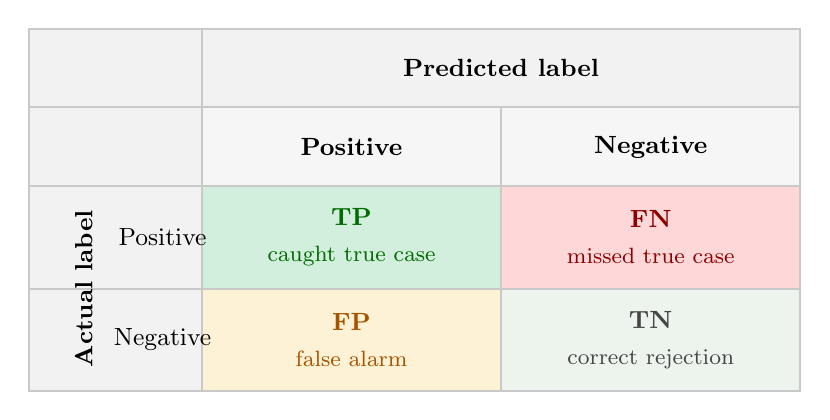
\begin{tikzpicture}[x=1cm, y=1cm, font=\small]
%%
%% Column x-boundaries:  0 | 2.2 | 6.0 | 9.8
%%   row-label column     0   –  2.2  (center x = 1.1)
%%   predicted positive  2.2  –  6.0  (center x = 4.1)
%%   predicted negative  6.0  –  9.8  (center x = 7.9)
%%
%% Row y-boundaries:  0 | 1.3 | 2.6 | 3.6 | 4.6
%%   actual-negative   0.0  – 1.3  (center y = 0.65)
%%   actual-positive   1.3  – 2.6  (center y = 1.95)
%%   sub-header        2.6  – 3.6  (center y = 3.10)
%%   main header       3.6  – 4.6  (center y = 4.10)
%%
%% ── Fills ─────────────────────────────────────────────────────────────────
\fill[gray!10]  (0,0)    rectangle (2.2,4.6);   % row-label column
\fill[gray!10]  (2.2,3.6) rectangle (9.8,4.6);  % main header
\fill[gray!7]   (2.2,2.6) rectangle (9.8,3.6);  % sub-header row
\fill[c2tpBg]   (2.2,1.3) rectangle (6.0,2.6);  % TP cell
\fill[c2fnBg]   (6.0,1.3) rectangle (9.8,2.6);  % FN cell
\fill[c2fpBg]   (2.2,0)   rectangle (6.0,1.3);  % FP cell
\fill[c2tnBg]   (6.0,0)   rectangle (9.8,1.3);  % TN cell
%% ── Grid lines ────────────────────────────────────────────────────────────
\draw[gray!42, line width=0.75pt] (0,0) rectangle (9.8,4.6);  % outer border
\draw[gray!42, line width=0.75pt] (2.2,0) -- (2.2,4.6);       % label | data
\draw[gray!42, line width=0.75pt] (6.0,0) -- (6.0,3.6);       % pred-col divider
\draw[gray!42, line width=0.75pt] (0,3.6) -- (9.8,3.6);       % main header base
\draw[gray!42, line width=0.75pt] (0,2.6) -- (9.8,2.6);       % sub-header base
\draw[gray!42, line width=0.75pt] (0,1.3) -- (9.8,1.3);       % data row divider
%% ── Main header ───────────────────────────────────────────────────────────
\node[font=\small\bfseries] at (6.0, 4.1) {Predicted label};
%% ── Column sub-headers (each centered in its column) ─────────────────────
\node[font=\small\bfseries] at (4.1, 3.1) {Positive};
\node[font=\small\bfseries] at (7.9, 3.1) {Negative};
%% ── Row labels ────────────────────────────────────────────────────────────
\node[rotate=90, font=\small\bfseries] at (0.7, 1.3) {Actual label};
\node[font=\small] at (1.7, 1.95) {Positive};
\node[font=\small] at (1.7, 0.65) {Negative};
%% ── Data cells ────────────────────────────────────────────────────────────
\node[align=center, text=green!42!black]  at (4.1, 1.95)
    {\textbf{TP}\\[2pt]\footnotesize caught true case};
\node[align=center, text=red!55!black]    at (7.9, 1.95)
    {\textbf{FN}\\[2pt]\footnotesize missed true case};
\node[align=center, text=orange!65!black] at (4.1, 0.65)
    {\textbf{FP}\\[2pt]\footnotesize false alarm};
\node[align=center, text=gray!55!black]   at (7.9, 0.65)
    {\textbf{TN}\\[2pt]\footnotesize correct rejection};
\end{tikzpicture}%
}
\caption{The confusion matrix is the bookkeeping layer between predicted scores and thresholded claims. Once a decision rule turns scores into positive or negative decisions, these counts determine what the metric rewards.}
\label{fig:confusion-matrix}
\end{figure}

From these counts we obtain common metrics:
\[
\text{Accuracy} = \frac{TP + TN}{TP + TN + FP + FN},
\]
\begin{align*}
\text{Precision} &= \frac{TP}{TP + FP}, \\[4pt]
\text{Recall} &= \frac{TP}{TP + FN},
\end{align*}
\[
\text{F1} = \frac{2 \cdot \text{Precision}\cdot \text{Recall}}
{\text{Precision} + \text{Recall}}.
\]

Accuracy measures overall correctness, but it can hide serious failures when one class is much more common than the other or when false positives and false negatives have very different costs. Precision asks, ``When the system says positive, how often is it right?'' Recall asks, ``Of the truly positive cases, how many did the system catch?'' F1 combines precision and recall into one number, but even that combination is only sensible when those two concerns matter in roughly balanced ways.

\begin{example}[Spam Filtering and Precision]
Spam filtering is naturally precision-sensitive. False positives are painful because legitimate messages get hidden or delayed. At Gmail scale, even a small false-positive rate can affect a large number of users \citep{gmail2023}. This is why spam systems are rarely judged by accuracy alone.
\end{example}

\begin{example}[Medical Screening and Recall]
The metric emphasis changes when false negatives are costly. The CDC notes that rapid influenza diagnostic tests often have sensitivities around 50--70\% and specificities around 90--95\%; here sensitivity means how often true cases are caught, and specificity means how often true negative cases are correctly rejected, that is $\mathrm{TN}/(\mathrm{TN}+\mathrm{FP})$ \citep{cdc_ridt}. The false positive rate is $\mathrm{FP}/(\mathrm{FP}+\mathrm{TN})$, so it is just $1-\text{specificity}$. A stricter threshold may reduce false alarms but miss too many real cases.
\end{example}

\begin{example}[Why Accuracy Can Fail Under Imbalance]
Imagine a screening dataset with $950$ negative cases and $50$ positive cases. A useless classifier that predicts ``negative'' for every person achieves
\[
\text{Accuracy} = \frac{950}{1000} = 95\%.
\]
That number sounds strong until we inspect recall. Because the classifier never predicts positive, it has
\[
TP=0,\quad FN=50,\quad \text{Recall}=0.
\]
The model is accurate only because the majority class dominates the dataset. This kind of skew, called class imbalance, makes accuracy an unsafe default.
\end{example}

\section{Training Loss as the Quantity Optimized During Learning}

Once the reported behavior is clear, training losses make more sense. A learning algorithm needs a rule for preferring one prediction over another during optimization, meaning during the process of adjusting the model to reduce error on the training data. That role is played by a loss function. This is the chapter's first separation: the number that teaches the model is not automatically the number that justifies the system.

\begin{definition}[Loss Function]
A loss function $\ell(y,\hat{y})$ measures how bad a prediction $\hat{y}$ is when the desired output is $y$. Smaller values are better, and a value of zero usually represents a perfect prediction.
\end{definition}

If a dataset contains $n$ training examples, a standard training objective is the average loss:
\[
\mathcal{L}_{\text{train}}(\theta) = \frac{1}{n} \sum_{i=1}^{n} \ell \bigl(y_i, f_\theta(x_i)\bigr).
\]
This quantity is often called the \emph{empirical risk}, meaning the average observed loss on the training sample.

\begin{definition}[Empirical Risk]
Empirical risk is the average loss measured on the observed training sample. It is called ``empirical'' because it is computed from available data rather than from the full unknown distribution of future examples.
\end{definition}

The wording matters. Empirical risk lives on the sample we have, not on the world we care about. This is why a low training loss is necessary but not sufficient.

\begin{prereqbridge}
If the summation notation looks dense, read the formula for empirical risk as ``compute the loss on every training example, add the losses together, and divide by the number of examples.''
\end{prereqbridge}

In the next table, \emph{log loss} means a probability-based penalty that grows when the model is confidently wrong.

\begin{table}[t]
\centering
\small
\setlength{\tabcolsep}{3pt}
\begin{tabular}{@{}>{\raggedright\arraybackslash}p{1.61cm}>{\raggedright\arraybackslash}p{2.1cm}>{\raggedright\arraybackslash}p{2.17cm}>{\raggedright\arraybackslash}p{4.27cm}@{}}
\toprule
Task & Training objective & Reporting metric & Why not identical? \\
\midrule
Spam filtering & Log loss on spam probabilities & Precision, recall, and false-positive behavior & Training needs a smooth probability loss; deployment cares about protecting inboxes without hiding wanted mail \\
Screening or triage & Probability loss or extra penalty for missed cases & Recall or sensitivity plus false-positive burden & The real question is often ``how many true cases are caught?'' rather than ``what is the average training loss?'' \\
Probabil\-ity forecasts & Probability loss rewarding honest confidence & Calibration and predicted-versus-observed plots & The model is used for its probabilities, so honest confidence matters more than one thresholded label \\
Ranking or retrieval & A training loss over item scores & Success among the top $k$ outputs or user success rate & The loss is chosen for optimization, but the user experiences only the ordered outputs \\
\bottomrule
\end{tabular}
\caption{Losses are for learning. Metrics are for claims. A good metric-and-action worksheet should explain why the optimized quantity and the reported quantity are not identical.}
\label{tab:loss-vs-metric}
\end{table}

\subsection{Regression Losses}

When the target is numeric, two common losses are mean squared error and mean absolute error:
\[
\text{MSE} = \frac{1}{n}\sum_{i=1}^{n}(y_i - \hat{y}_i)^2,
\qquad
\text{MAE} = \frac{1}{n}\sum_{i=1}^{n}|y_i - \hat{y}_i|.
\]

Mean squared error punishes large mistakes more strongly because the error is squared. Mean absolute error treats error more linearly. Neither is universally better. The choice should reflect what kinds of misses the application can tolerate.

\begin{practicalnote}
If a model were forced to predict one constant value for every example, squared error would pull that constant toward the average target, while absolute error would pull it toward a median or middle case. Students should read this as a modeling judgment first: squared loss reacts more strongly to outliers, while absolute loss is more resistant.
\end{practicalnote}

\begin{example}[One Constant Prediction]
Suppose three apartments sold for \$200{,}000, \$220{,}000, and \$600{,}000. If a model were forced to predict one constant price for every apartment, squared error would be pulled upward by the expensive outlier, while absolute error would prefer a middle value closer to the typical case. The intuition comes first: MSE leans harder toward the average when large misses matter a lot, while MAE is more resistant to one extreme example.
\end{example}

\begin{mathlens}
The example above can be stated sharply when the model is forced to predict one constant value for every example.

\begin{theorem}[Best Constant Predictor]
Let $y_1,\ldots,y_n$ be observed target values, and suppose the prediction is restricted to a single constant $c$.
\begin{enumerate}[leftmargin=*,label=\arabic*.]
\item The value of $c$ that minimizes $\frac{1}{n}\sum_{i=1}^{n}(y_i-c)^2$ is the sample mean $\bar{y}=\frac{1}{n}\sum_{i=1}^{n} y_i$.
\item The value of $c$ that minimizes $\frac{1}{n}\sum_{i=1}^{n}|y_i-c|$ is any sample median: when the targets are sorted, any middle observed value for odd $n$, or any value between the two middle order statistics for even $n$.
\end{enumerate}
\end{theorem}

\begin{proof}[Proof Sketch]
For squared error, expand $(y_i-c) = (y_i-\bar{y}) + (\bar{y}-c)$. After summing, the cross-term disappears and we get
\[
\sum_{i=1}^{n}(y_i-c)^2 = \sum_{i=1}^{n}(y_i-\bar{y})^2 + n(\bar{y}-c)^2,
\]
so the minimum occurs at $c=\bar{y}$. For absolute error, if $c$ sits to the left of the median interval, more than half of the sorted targets lie to its right, so moving $c$ slightly right decreases more distances than it increases. The symmetric argument applies when $c$ lies to the right of that interval. When $n$ is even, this leaves a flat interval between the two middle order statistics on which the total absolute deviation is constant. That is why any median minimizes total absolute deviation.
\end{proof}
\end{mathlens}

\begin{practicalnote}
This theorem is one reason squared error reacts strongly to outliers while absolute error is more resistant. They are not just different penalties. They prefer different notions of ``center.''
\end{practicalnote}

\begin{figure}[t]
\centering
\definecolor{c2maeBl}{RGB}{56,103,170}
\definecolor{c2mseOr}{RGB}{184,92,16}
\resizebox{\linewidth}{!}{%
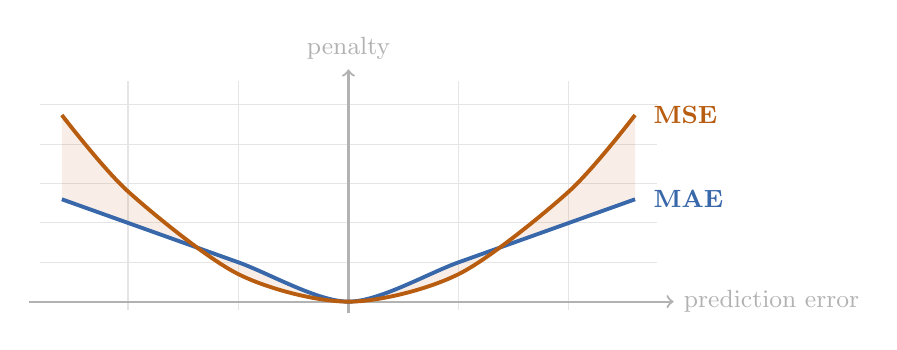
\begin{tikzpicture}[x=1.4cm, y=1.0cm, font=\small]
%% ── Light grid ───────────────────────────────────────────────────────────
\foreach \x in {-2,-1,1,2}
    \draw[gray!20, line width=0.4pt] (\x,-0.1) -- (\x,2.8);
\foreach \y in {0.5,1.0,1.5,2.0,2.5}
    \draw[gray!20, line width=0.4pt] (-2.8,\y) -- (2.8,\y);
%% ── Axes ─────────────────────────────────────────────────────────────────
\draw[->, gray!60, thick] (-2.9,0) -- (2.95,0) node[right] {prediction error};
\draw[->, gray!60, thick] (0,-0.15) -- (0,2.95) node[above] {penalty};
%% ── Fill between curves (shows MSE excess over MAE) ──────────────────────
\fill[c2mseOr, opacity=0.10]
    plot[smooth] coordinates {(-2.6,1.30)(-2.0,1.00)(-1.0,0.50)(0,0)(1.0,0.50)(2.0,1.00)(2.6,1.30)}
    -- plot[smooth] coordinates {(2.6,2.37)(2.0,1.40)(1.0,0.35)(0,0)(-1.0,0.35)(-2.0,1.40)(-2.6,2.37)}
    -- cycle;
%% ── MAE curve (linear, blue) ─────────────────────────────────────────────
\draw[c2maeBl, line width=1.4pt]
    plot[smooth] coordinates
    {(-2.6,1.30) (-2.0,1.00) (-1.0,0.50) (0,0) (1.0,0.50) (2.0,1.00) (2.6,1.30)};
%% ── MSE curve (quadratic, orange) ────────────────────────────────────────
\draw[c2mseOr, line width=1.4pt]
    plot[smooth] coordinates
    {(-2.6,2.37) (-2.0,1.40) (-1.0,0.35) (0,0) (1.0,0.35) (2.0,1.40) (2.6,2.37)};
%% ── Legend labels: placed to the right of curve endpoints ────────────────
\node[c2maeBl, anchor=west, font=\small\bfseries] at (2.68,1.30) {MAE};
\node[c2mseOr, anchor=west, font=\small\bfseries] at (2.68,2.37) {MSE};
\end{tikzpicture}%
}
\caption{MAE grows linearly with the error size, while MSE punishes larger misses much more aggressively. That shape difference explains much of the practical tradeoff.}
\label{fig:mse-vs-mae}
\end{figure}

\begin{example}[House Price Prediction]
If a model predicts house prices, an error of \$200{,}000 is often more serious than two errors of \$100{,}000. Squared error reflects that intuition by penalizing the larger miss more aggressively. In other settings, such as predicting waiting times or delivery delays, a more linear penalty may be easier to justify.
\end{example}

\subsection{Classification Losses}

In classification, the output is a class label or a probability distribution over classes. A conceptually simple loss for a yes-or-no task is the zero-one loss:
\[
\ell(y,\hat{y}) =
\begin{cases}
0 & \text{if } y=\hat{y},\\
1 & \text{if } y\neq \hat{y}.
\end{cases}
\]
This definition is conceptually simple, but it is usually not optimized directly because many common training algorithms work best with losses that change smoothly as the prediction changes.

Instead, classification models are often trained with cross-entropy, also called log loss. For a classifier in a yes-or-no task that predicts a probability $p$ for the positive class, the loss on one example is
\[
\ell(y,p) = -\bigl(y \log p + (1-y)\log(1-p)\bigr).
\]
This loss becomes small when the model assigns high probability to the correct class and large when it is confident and wrong.

\begin{mathlens}
If $y=1$, then $\ell=-\log p$; if $y=0$, then $\ell=-\log(1-p)$. So as the model becomes more confident in the wrong class, the penalty rises fast because $\log z \to -\infty$ as $z \to 0^+$. For a concrete anchor, predicting $p=0.99$ for a negative case gives $\ell=-\log(0.01)\approx 4.61$, while an uncertain $p=0.5$ gives only $\ell\approx 0.69$.
\end{mathlens}

\begin{figure}[t]
\centering
\definecolor{c2cautBg}{RGB}{220,233,251}
\definecolor{c2confBg}{RGB}{210,238,220}
\resizebox{\linewidth}{!}{%
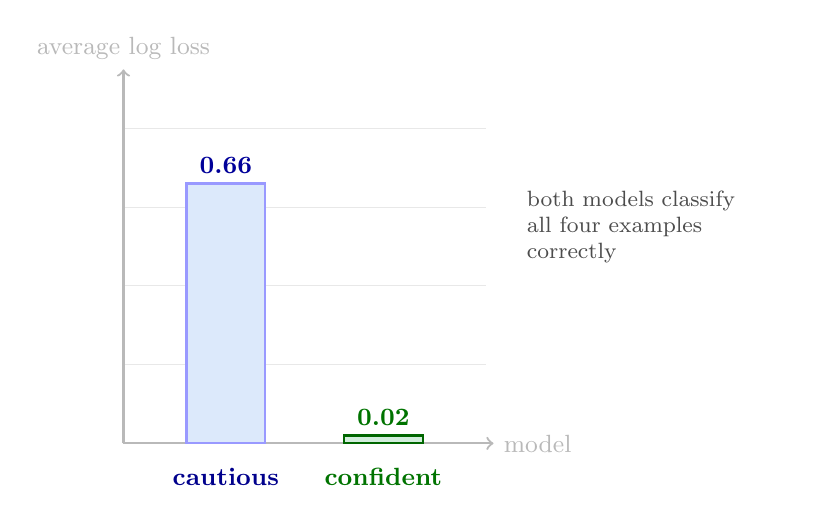
\begin{tikzpicture}[x=1cm, y=5cm, font=\small]
%% ── Light grid ───────────────────────────────────────────────────────────
\foreach \y in {0.2,0.4,0.6,0.8}
    \draw[gray!18, line width=0.4pt] (0,\y) -- (4.6,\y);
%% ── Axes ─────────────────────────────────────────────────────────────────
\draw[->, gray!55, thick] (0,0) -- (4.7,0) node[right] {model};
\draw[->, gray!55, thick] (0,0) -- (0,0.95) node[above] {average log loss};
%% ── Bars ─────────────────────────────────────────────────────────────────
\filldraw[fill=c2cautBg, draw=blue!40, line width=0.8pt]
    (0.8,0) rectangle (1.8,0.66);
\filldraw[fill=c2confBg, draw=green!40!black, line width=0.8pt]
    (2.8,0) rectangle (3.8,0.02);
%% ── Bar value labels ─────────────────────────────────────────────────────
\node[above, font=\small\bfseries, blue!60!black]  at (1.3,0.66) {0.66};
\node[above, font=\small\bfseries, green!45!black] at (3.3,0.02) {0.02};
%% ── Axis tick labels ─────────────────────────────────────────────────────
\node[align=center, font=\small\bfseries, blue!55!black]  at (1.3,-0.085) {cautious};
\node[align=center, font=\small\bfseries, green!45!black] at (3.3,-0.085) {confident};
%% ── Annotation (right side, clear of the 0.67 label) ────────────────────
\node[align=left, text width=3.2cm, font=\footnotesize, gray!60!black,
      anchor=west]
    at (5.0,0.55) {both models classify\\all four examples\\correctly};
\end{tikzpicture}%
}
\caption{Accuracy can hide major differences in confidence. A cautious model and a confident model may both be perfectly accurate while having very different log loss.}
\label{fig:same-accuracy-different-logloss}
\end{figure}

\begin{table}[t]
\centering
\small
\setlength{\tabcolsep}{5pt}
\begin{tabular}{>{\centering}p{1.38cm}>{\centering}p{1.4cm}>{\centering}p{2.35cm}>{\centering}p{2.35cm}>{\centering\arraybackslash}p{1.52cm}}
\toprule
Example & True label & Cautious $p(y{=}1{\mid}x)$ & Confident $p(y{=}1{\mid}x)$ & Correct? \\
\midrule
1 & 1 & 0.51 & 0.99 & both correct \\
2 & 1 & 0.52 & 0.98 & both correct \\
3 & 0 & 0.49 & 0.02 & both correct \\
4 & 0 & 0.48 & 0.01 & both correct \\
\bottomrule
\end{tabular}
\caption{The final labels are identical, but the probabilistic quality is not. Log loss rewards the model that is confidently correct, not merely barely correct.}
\label{tab:log-loss-comparison}
\end{table}

\begin{example}[Why Confidence Matters at Scale]
Google reports that Gmail's AI-powered defenses block nearly 15 billion unwanted messages per day and stop more than 99.9\% of spam, phishing, and malware from reaching inboxes \citep{gmail2023}. At that scale, confidence matters because downstream systems use those probabilities for ranking, quarantine decisions, and human-review queues.
\end{example}

\begin{thinkingtool}
\textbf{Counterexample first.} Before trusting one headline metric, try to construct two models that tie on that metric but differ in decision value. If you can build such a pair, the metric is not sufficient by itself.
\end{thinkingtool}

\begin{practicalnote}
When classes are imbalanced, the average loss can be dominated by the majority class. One common remedy is to weight the loss: multiply the per-example loss by a factor that is larger for minority-class examples. If the positive class appears in only 5\% of training examples, an inverse-frequency weight would be $w_+ = 20$. Class-weighted cross-entropy is the standard version:
\[
\mathcal{L} = -\frac{1}{n}\sum_{i=1}^{n} w_{y_i}\bigl[y_i\log p_i + (1-y_i)\log(1-p_i)\bigr],
\]
where $w_1 > w_0$ reflects the higher cost of ignoring the rarer class. This is a training-time choice that complements the deployment-time threshold and cost-matrix choices discussed in Section~\ref{sec:from-score-to-action}. Adjusting the loss and adjusting the threshold are two different levers; in practice, teams often use both.
\end{practicalnote}

\begin{warningbox}
If you report only the optimized training loss, you may hide the behavior that matters for the real decision. A system can improve its loss while leaving the practically important metric unchanged or even worse.
\end{warningbox}

\section{From Score to Action: Threshold, Ranking, and Abstention}
\label{sec:from-score-to-action}

Up to this point, the chapter has asked what behavior should be reported. But teams do not act on reported numbers alone. They act on policies built from scores. Many models therefore produce scores or probabilities first, and a separate rule turns them into action. That rule may involve a threshold, a top-$k$ ranking, meaning ``take the highest $k$ scores,'' or an abstention rule, meaning a rule that withholds automatic action on uncertain cases and sends them to human review. This is the chapter's second separation: even a well-chosen metric is incomplete until the score is attached to an operational policy.

\begin{thinkingtool}
\textbf{Threshold as policy.} A threshold is not a cleanup detail after training. It encodes a decision about missed cases, false alarms, review capacity, and intervention cost.
\end{thinkingtool}

\begin{decisionbox}
\textbf{Threshold, top-$k$, or abstain?}
\begin{itemize}[leftmargin=*]
\item Use a \textbf{threshold} when each case can be acted on independently and crossing one risk boundary should trigger the same kind of action.
\item Use \textbf{top-$k$ ranking} when capacity is fixed and only the highest-scoring cases can be reviewed or contacted in each cycle.
\item Use \textbf{abstention} when the system should act automatically only on clearly supported cases and defer borderline cases to human review.
\end{itemize}
The model score can stay the same while the policy changes. Same model, different policy.
\end{decisionbox}

\subsection{Threshold Tradeoffs}

Suppose a spam detector assigns the following probabilities to eight messages.

\begin{table}[t]
\centering
\begin{tabular}{>{\centering}p{1.4cm}>{\centering}p{1.4cm}>{\centering}p{2.6cm}>{\centering\arraybackslash}p{3.7cm}}
\toprule
Message & True label & Predicted spam probability & Positive at $0.3$ / $0.5$ / $0.7$ \\
\midrule
1 & 1 & 0.95 & yes / yes / yes \\
2 & 1 & 0.81 & yes / yes / yes \\
3 & 1 & 0.64 & yes / yes / no \\
4 & 0 & 0.58 & yes / yes / no \\
5 & 1 & 0.41 & yes / no / no \\
6 & 0 & 0.35 & yes / no / no \\
7 & 0 & 0.18 & no / no / no \\
8 & 0 & 0.07 & no / no / no \\
\bottomrule
\end{tabular}
\caption{A tiny thresholding example for binary classification metrics.}
\label{tab:threshold-example}
\end{table}

At threshold $0.3$, Messages 1 through 6 are predicted positive. The confusion counts are
\[
TP=4,\quad FP=2,\quad FN=0,\quad TN=2,
\]
so the metrics become
\[
\text{Accuracy}=\frac{4+2}{8}=0.75,
\qquad
\text{Precision}=\frac{4}{4+2}\approx 0.67,
\]
\[
\text{Recall}=\frac{4}{4+0}=1.00,
\qquad
\text{F1}\approx 0.80.
\]

At threshold $0.5$, Messages 1 through 4 are predicted positive:
\[
TP=3,\quad FP=1,\quad FN=1,\quad TN=3,
\]
which gives
\begin{align*}
\text{Accuracy} &= 0.75, & \text{Precision} &= 0.75, \\
\text{Recall} &= 0.75, & \text{F1} &= 0.75.
\end{align*}

At threshold $0.7$, only Messages 1 and 2 remain positive:
\[
TP=2,\quad FP=0,\quad FN=2,\quad TN=4,
\]
so
\begin{align*}
\text{Accuracy} &= 0.75, & \text{Precision} &= 1.00, \\
\text{Recall} &= 0.50, & \text{F1} &\approx 0.67.
\end{align*}

\begin{figure}[t]
\centering
\definecolor{c2precBl}{RGB}{56,103,170}
\definecolor{c2recOr}{RGB}{184,92,16}
\resizebox{\linewidth}{!}{%
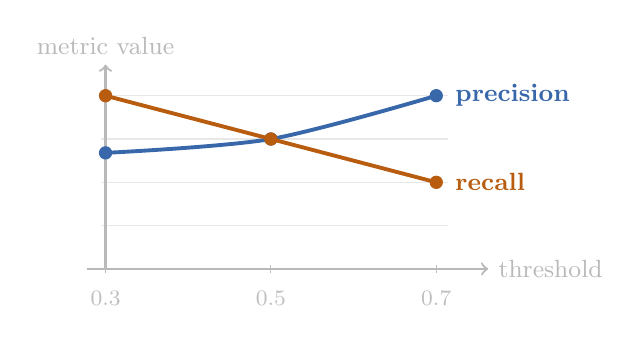
\begin{tikzpicture}[x=3.0cm, y=2.2cm, font=\small]
%% ── Light grid ───────────────────────────────────────────────────────────
\foreach \y in {0.25,0.50,0.75,1.00}
    \draw[gray!18, line width=0.4pt] (0.28,\y) -- (1.75,\y);
%% ── Axes ─────────────────────────────────────────────────────────────────
\draw[->, gray!55, thick] (0.22,0) -- (1.92,0) node[right] {threshold};
\draw[->, gray!55, thick] (0.30,0) -- (0.30,1.18) node[above] {metric value};
%% ── Tick marks ───────────────────────────────────────────────────────────
\foreach \x/\lbl in {0.3/0.3, 1.0/0.5, 1.7/0.7}
    \draw[gray!50] (\x,0.025) -- (\x,-0.025) node[below=3pt, font=\footnotesize] {\lbl};
%% ── Precision curve (blue, rising) ──────────────────────────────────────
\draw[c2precBl, line width=1.4pt]
    plot[smooth] coordinates {(0.3,0.67) (1.0,0.75) (1.7,1.00)};
\filldraw[c2precBl] (0.3,0.67) circle (2.2pt);
\filldraw[c2precBl] (1.0,0.75) circle (2.2pt);
\filldraw[c2precBl] (1.7,1.00) circle (2.2pt);
%% ── Recall curve (orange, falling) ──────────────────────────────────────
\draw[c2recOr, line width=1.4pt]
    plot[smooth] coordinates {(0.3,1.00) (1.0,0.75) (1.7,0.50)};
\filldraw[c2recOr] (0.3,1.00) circle (2.2pt);
\filldraw[c2recOr] (1.0,0.75) circle (2.2pt);
\filldraw[c2recOr] (1.7,0.50) circle (2.2pt);
%% ── Legend labels: right of last data point to avoid curve overlap ────────
\node[c2precBl, anchor=west, font=\small\bfseries] at (1.74,1.00) {precision};
\node[c2recOr,  anchor=west, font=\small\bfseries] at (1.74,0.50) {recall};
\end{tikzpicture}%
}
\caption{The threshold sweep makes the tradeoff visible: stricter thresholds usually raise precision and lower recall. The underlying model stays the same. Only the policy changes.}
\label{fig:threshold-sweep}
\end{figure}

This is why metric choice and threshold choice cannot be separated. Accuracy stayed the same across all three thresholds, but the operating behavior changed substantially.

The arithmetic is simple enough to reproduce with basic Python only.

\begin{codeexample}[caption={A pure-Python threshold sweep}]
scores = [0.95, 0.81, 0.64, 0.58, 0.41, 0.35, 0.18, 0.07]
labels = [1,    1,    1,    0,    1,    0,    0,    0]

def metrics_at_threshold(scores, labels, threshold):
    tp = fp = fn = tn = 0

    for score, label in zip(scores, labels):
        prediction = 1 if score >= threshold else 0
        if prediction == 1 and label == 1:
            tp += 1
        elif prediction == 1 and label == 0:
            fp += 1
        elif prediction == 0 and label == 1:
            fn += 1
        else:
            tn += 1

    accuracy = (tp + tn) / len(labels)
    precision = tp / (tp + fp) if tp + fp else 0.0
    recall = tp / (tp + fn) if tp + fn else 0.0
    f1 = 0.0 if precision + recall == 0 else 2 * precision * recall / (precision + recall)
    return tp, fp, fn, tn, accuracy, precision, recall, f1

for threshold in [0.3, 0.5, 0.7]:
    tp, fp, fn, tn, accuracy, precision, recall, f1 = metrics_at_threshold(
        scores, labels, threshold
    )
    print(
        threshold,
        (tp, fp, fn, tn),
        round(accuracy, 2),
        round(precision, 2),
        round(recall, 2),
        round(f1, 2),
    )
\end{codeexample}

\begin{practicalnote}
This kind of tiny script belongs in the book because it exposes the mechanism. The labs can use libraries and larger datasets; the chapter code should make the evaluation arithmetic impossible to hide.
\end{practicalnote}

\subsection{Cost Matrices and Threshold Selection}

Threshold choice becomes much clearer when we stop asking which threshold has the nicest generic metric and start asking what the downstream action costs.

Suppose first that the system is a medical triage screen where a false negative is much worse than a false positive because a missed urgent case may delay treatment. If we assign cost $6$ to each false negative and cost $1$ to each false positive, then the total decision cost on the running eight-message threshold example would be:
\begin{align*}
\text{cost}_{0.3} &= 2(1)+0(6)=2, \\
\text{cost}_{0.5} &= 1(1)+1(6)=7, \\
\text{cost}_{0.7} &= 0(1)+2(6)=12.
\end{align*}
Under that policy, the lowest threshold is best because misses are expensive.

Now reverse the deployment story. Suppose the system is a strict inbox-protection tool where quarantining wanted mail is much more harmful than letting one nuisance message through. If a false positive costs $5$ and a false negative costs $1$, then
\begin{align*}
\text{cost}_{0.3} &= 2(5)+0(1)=10, \\
\text{cost}_{0.5} &= 1(5)+1(1)=6, \\
\text{cost}_{0.7} &= 0(5)+2(1)=2.
\end{align*}
Under that policy, the highest threshold is best because false alarms are expensive.

\begin{table}[t]
\centering
\small
\setlength{\tabcolsep}{4pt}
\begin{tabular}{@{}>{\raggedright\arraybackslash}p{1.73cm}>{\centering\arraybackslash}p{0.99cm}>{\centering\arraybackslash}p{0.99cm}>{\centering\arraybackslash}p{2.97cm}>{\centering\arraybackslash}p{2.97cm}@{}}
\toprule
Threshold & FP & FN & Cost if FN is severe $(FP=1,\ FN=6)$ & Cost if FP is severe $(FP=5,\ FN=1)$ \\
\midrule
$0.3$ & $2$ & $0$ & $2$ & $10$ \\
$0.5$ & $1$ & $1$ & $7$ & $6$ \\
$0.7$ & $0$ & $2$ & $12$ & $2$ \\
\bottomrule
\end{tabular}
\caption{The same score distribution can imply different thresholds once the action costs change. Threshold choice is therefore a policy choice, not a universal mathematical truth.}
\label{tab:threshold-cost-matrix}
\end{table}

This is the operational meaning of ``threshold as policy.'' The score has not changed. The ranking has not changed. Only the consequence model changed, and that alone was enough to reverse the preferred threshold.

\begin{mathlens}
Let $q=P(y=1\mid x)$ be a calibrated probability for a single case. If we predict positive, the expected cost is $C_{FP}(1-q)$; if we predict negative, it is $C_{FN}q$. Choose positive when
\[
C_{FP}(1-q)\le C_{FN}q
\quad\Rightarrow\quad
q\ge \frac{C_{FP}}{C_{FP}+C_{FN}}.
\]
So the reusable threshold rule is $t^*=\frac{C_{FP}}{C_{FP}+C_{FN}}$ for calibrated probabilities, and the threshold moves directly with the cost ratio.
\end{mathlens}

\begin{decisionbox}
Do not ask which threshold maximizes one generic metric until you have written down what false positives, false negatives, abstentions, or review load actually cost in the deployment workflow. If misses are costlier, emphasize recall; if false alarms are costlier, emphasize precision.
\end{decisionbox}

\subsection{Ranking Under a Fixed Budget}

Suppose a university builds a model that predicts the probability that a student will miss the first two major deadlines in a programming course. The output is a probability, not a final judgment. Staff can contact at most five students this week.

\begin{table}[t]
\centering
\begin{tabular}{>{\centering}p{1.4cm}>{\centering}p{1.7cm}>{\centering}p{2.3cm}>{\centering\arraybackslash}p{3.7cm}}
\toprule
Student & Predicted risk & Missed deadlines? & Flagged at $0.3$ / $0.5$ / $0.7$ \\
\midrule
S1 & 0.92 & 1 & yes / yes / yes \\
S2 & 0.84 & 1 & yes / yes / yes \\
S3 & 0.78 & 1 & yes / yes / yes \\
S4 & 0.66 & 0 & yes / yes / no \\
S5 & 0.61 & 1 & yes / yes / no \\
S6 & 0.54 & 0 & yes / yes / no \\
S7 & 0.47 & 1 & yes / no / no \\
S8 & 0.39 & 0 & yes / no / no \\
S9 & 0.33 & 1 & yes / no / no \\
S10 & 0.22 & 0 & no / no / no \\
S11 & 0.14 & 0 & no / no / no \\
S12 & 0.08 & 0 & no / no / no \\
\bottomrule
\end{tabular}
\caption{A small threshold-setting example for student support. The staffing constraint forces the evaluation to include operational capacity, not only abstract metrics.}
\label{tab:student-threshold-example}
\end{table}

\begin{table}[t]
\centering
\small
\setlength{\tabcolsep}{5pt}
\begin{tabular}{>{\centering}p{1.0cm}>{\centering}p{1.4cm}>{\centering}p{1.45cm}>{\centering}p{1.1cm}>{\centering}p{0.8cm}>{\centering\arraybackslash}p{2.85cm}}
\toprule
Policy & Flagged & Precision & Recall & F1 & Within budget? \\
\midrule
$0.30$ & 9 & $6/9 \approx 0.67$ & $6/6 = 1.00$ & 0.80 & no \\
$0.50$ & 6 & $4/6 \approx 0.67$ & $4/6 \approx 0.67$ & 0.67 & almost, but still too many \\
$0.70$ & 3 & $3/3 = 1.00$ & $3/6 = 0.50$ & 0.67 & yes, but leaves capacity unused \\
Top 5 scores & 5 & $4/5 = 0.80$ & $4/6 \approx 0.67$ & 0.73 & yes, exactly \\
\bottomrule
\end{tabular}
\caption{Threshold or ranking choice is partly a resource-allocation choice. The metric story changes once the operational budget is included.}
\label{tab:student-threshold-summary}
\end{table}

This is a more realistic version of threshold selection than ``pick the threshold with the highest score.'' A threshold of $0.30$ catches every at-risk student in this toy set, but it flags nine students when the staff can contact only five. A threshold of $0.70$ is very precise, but it misses half of the struggling students and leaves scarce support capacity unused. The top-five ranking policy uses the full support budget exactly and keeps four of the six at-risk students in scope.

The operational conclusion is not that one threshold is mathematically correct. It is that policy choice must be made together with capacity planning. In a real system, the university might use the top five scores rather than a fixed threshold, or it might add a review step for students near the boundary. Ranking policies become natural when intervention budget is fixed in advance.

\subsection{Top-\texorpdfstring{$k$}{k} and Retrieval Metrics}

When the system acts on a short ranked list, the top of the list matters more than average behavior over the whole candidate set. This is common in search, recommendation, document retrieval, limited-capacity triage, and review queues. In these settings, threshold metrics alone can miss the central question: how useful is the short list that users or staff will actually see?

Two common quantities are
\begin{align*}
\text{Precision@}k &= \frac{\text{relevant items in the top }k}{k}, \\
\text{Recall@}k &= \frac{\text{relevant items in the top }k}{\text{all relevant items}}.
\end{align*}
Precision@k asks how clean the exposed list is. Recall@k asks how much of the useful material the list managed to capture. If there is usually one best item, such as one authoritative policy passage or one best search result, then the position of the \emph{first} relevant result matters too. Information-retrieval texts often summarize that idea with reciprocal rank or mean reciprocal rank \citep{manning2008}.

\begin{example}[A Tiny Retrieval Ranking]
Suppose a policy-search system returns five passages, the first relevant passage appears at rank $2$, and two of the top five passages are relevant. If the collection contains three relevant passages in total, then $\text{Precision@}5 = 2/5 = 0.40$ and $\text{Recall@}5 = 2/3 \approx 0.67$, while the reciprocal rank is $1/2 = 0.5$. The system did not put the best evidence first, but it still surfaced useful material near the top of the list.
\end{example}

The practical lesson is that thresholds answer ``act or not?'' while ranking metrics answer ``how good is the short list we expose?'' Retrieval systems and recommender lists are both top-of-list problems in this sense, even if their downstream actions differ.

\subsection{Abstention and Review}

Some systems should not force every score into an automatic yes-or-no action. A model may abstain on borderline cases and route them to a human reviewer. This is especially sensible when the cost of a wrong automatic action is high or when the model's probabilities are not trustworthy enough for full automation. Chapter 13 returns to this systems view in detail, but the judgment lesson already belongs here: sometimes the best policy is ``predict, but do not act automatically.''

\subsection{ROC and Precision-Recall Curves}

Thresholds are often explored across a whole range rather than at one point. A receiver operating characteristic (ROC) curve plots true positive rate against false positive rate as the threshold changes. Here true positive rate is the same as recall, and false positive rate is the fraction of negative cases incorrectly flagged positive. A precision-recall (PR) curve plots precision against recall across thresholds. The ROC view is often useful when false positive rate is central. The PR view is often more informative when positive cases are rare and precision matters directly.

When positives are rare, ROC can still look deceptively healthy because the negative class dominates the denominator, while PR shows the burden of false positives directly through precision.

At Chapter 2 level, the main lesson is simple: these curves summarize \emph{families} of operating points rather than one operating point. Confusion matrices and ROC curves are standard tools in introductory AI and machine-learning courses, so the main job here is to interpret them in context rather than to re-derive them from scratch.

\begin{advancednote}
When there are more than two classes, the same logic still applies but the bookkeeping table gets larger. A multiclass confusion matrix has one row and one column per class. Macro-averaged metrics compute the quantity separately for each class and then average across classes, which gives rare classes equal weight. Micro-averaged metrics pool the class decisions first and then compute one global quantity, which gives common classes more influence. A news-topic classifier makes this distinction practical rather than theoretical.
\end{advancednote}

\begin{minimumtakeaway}
Metrics judge behavior, but policies decide what the system actually does. The same model score table can support a threshold, a fixed-budget top-$k$ rule, or an abstention-to-review workflow, so never report the score without the action rule that gives it meaning.
\end{minimumtakeaway}

\section{Confidence Quality: Calibration}

After thresholds and rankings, one more question remains. Sometimes a score is not used only to order cases. It is used as a statement of confidence. When that happens, we need to know whether the number means what it seems to mean. A model can discriminate well enough to order cases correctly and still be unreliable as a source of numerical confidence.

Calibration matters when a model's score is supposed to behave like confidence. A model is well calibrated if events predicted with probability $0.8$ occur about $80\%$ of the time. In this book's worldview, calibration is not optional decoration. Thresholds, abstention rules, review queues, and risk-based interventions behave better when the predicted probabilities can be interpreted honestly.

One standard scalar summary is the Brier score, the mean squared difference between predicted probability and observed outcome:
\[
\text{Brier} = \frac{1}{n}\sum_{i=1}^{n}(p_i - y_i)^2.
\]
Lower is better, though a reliability diagram still shows where the probability errors live.

Accuracy tells us whether labels were often right. Calibration tells us whether confidence itself can be trusted.

This is not just a theoretical concern. Modern neural networks can achieve strong classification accuracy while still being systematically overconfident \citep{guo2017}. A model that looks accurate at one threshold may still be unsafe to use as a probability estimator for intervention, triage, or automated action.

\begin{figure}[t]
\centering
\definecolor{c2overBg}{RGB}{254,237,215}
\definecolor{c2wellBg}{RGB}{220,233,251}
\resizebox{\linewidth}{!}{%
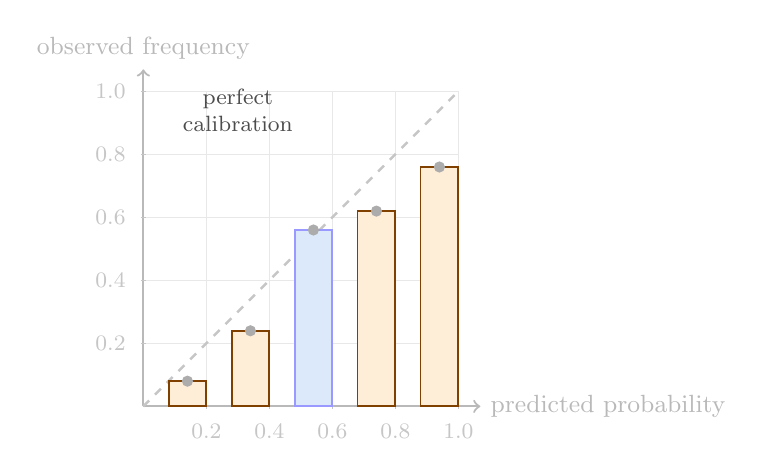
\begin{tikzpicture}[x=4.0cm, y=4.0cm, font=\small]
%% ── Light grid ───────────────────────────────────────────────────────────
\foreach \v in {0.2,0.4,0.6,0.8,1.0}
    \draw[gray!18, line width=0.4pt] (0,\v) -- (1.0,\v);
\foreach \v in {0.2,0.4,0.6,0.8,1.0}
    \draw[gray!18, line width=0.4pt] (\v,0) -- (\v,1.0);
%% ── Axes ─────────────────────────────────────────────────────────────────
\draw[->, gray!55, thick] (0,0) -- (1.07,0)
    node[right] {predicted probability};
\draw[->, gray!55, thick] (0,0) -- (0,1.07)
    node[above] {observed frequency};
%% ── Axis ticks ───────────────────────────────────────────────────────────
\foreach \v in {0.2,0.4,0.6,0.8,1.0} {
    \draw[gray!45] (\v,0.008) -- (\v,-0.008) node[below=2pt, font=\footnotesize] {\v};
    \draw[gray!45] (0.008,\v) -- (-0.008,\v) node[left=2pt,  font=\footnotesize] {\v};
}
%% ── Perfect-calibration diagonal ─────────────────────────────────────────
\draw[gray!45, dashed, line width=0.9pt] (0,0) -- (1,1);
%% ── Bars: orange=overconfident (obs < pred), blue=well-calibrated ────────
%% Bin 1: center=0.14, obs=0.08 < 0.14  → overconfident (orange)
\filldraw[fill=c2overBg, draw=orange!50!black, line width=0.7pt]
    (0.08,0) rectangle (0.20,0.08);
%% Bin 2: center=0.34, obs=0.24 < 0.34  → overconfident (orange)
\filldraw[fill=c2overBg, draw=orange!50!black, line width=0.7pt]
    (0.28,0) rectangle (0.40,0.24);
%% Bin 3: center=0.54, obs=0.56 > 0.54  → near-diagonal (blue)
\filldraw[fill=c2wellBg, draw=blue!40, line width=0.7pt]
    (0.48,0) rectangle (0.60,0.56);
%% Bin 4: center=0.74, obs=0.62 < 0.74  → overconfident (orange)
\filldraw[fill=c2overBg, draw=orange!50!black, line width=0.7pt]
    (0.68,0) rectangle (0.80,0.62);
%% Bin 5: center=0.94, obs=0.76 < 0.94  → overconfident (orange)
\filldraw[fill=c2overBg, draw=orange!50!black, line width=0.7pt]
    (0.88,0) rectangle (1.00,0.76);
%% ── Observed-frequency dots ──────────────────────────────────────────────
\filldraw[gray!65] (0.14,0.08) circle (1.8pt);
\filldraw[gray!65] (0.34,0.24) circle (1.8pt);
\filldraw[gray!65] (0.54,0.56) circle (1.8pt);
\filldraw[gray!65] (0.74,0.62) circle (1.8pt);
\filldraw[gray!65] (0.94,0.76) circle (1.8pt);
%% ── Legend ───────────────────────────────────────────────────────────────
\node[align=center, font=\footnotesize, gray!60!black]
    at (0.30,0.94) {perfect\\calibration};
\end{tikzpicture}%
}
\caption{A reliability diagram compares predicted probability with observed frequency. The dashed diagonal is ideal. Bars below the line indicate overconfident predictions.}
\label{fig:reliability-diagram}
\end{figure}

\begin{table}[t]
\centering
\scriptsize
\setlength{\tabcolsep}{3pt}
\begin{tabular}{p{1.35cm}p{0.9cm}p{1.45cm}p{0.8cm}p{1.15cm}p{1.55cm}}
\toprule
Bin & Cases & Avg.\ $p$ & Pos. & Obs.\ freq. & Interp. \\
\midrule
$[0.0,0.2)$ & $50$ & $0.14$ & $4$ & $4/50 = 0.08$ & over-conf. \\
$[0.2,0.4)$ & $50$ & $0.34$ & $12$ & $12/50 = 0.24$ & over-conf. \\
$[0.4,0.6)$ & $50$ & $0.54$ & $28$ & $28/50 = 0.56$ & close \\
$[0.6,0.8)$ & $50$ & $0.74$ & $31$ & $31/50 = 0.62$ & over-conf. \\
$[0.8,1.0]$ & $50$ & $0.94$ & $38$ & $38/50 = 0.76$ & over-conf. \\
\bottomrule
\end{tabular}
\caption{One concrete way to read a reliability diagram: bin the probabilities, average the prediction in each bin, count how many positives actually occurred, and compare the two numbers.}
\label{tab:calibration-bins}
\end{table}

\begin{practicalnote}
To build a reliability diagram by hand on a small example, use four steps: bin the predicted probabilities, compute the mean predicted probability in each bin, count the observed positives in that bin, and plot observed frequency against predicted probability. Table~\ref{tab:calibration-bins} is the hand-worked version of Figure~\ref{fig:reliability-diagram}.
\end{practicalnote}

\begin{sanitycheck}
If a bin has mean predicted probability $0.74$ but only $31$ of $50$ cases are positive, the model is overconfident in that region because $0.62 < 0.74$.
\end{sanitycheck}

\begin{example}[Weather Forecasting and Calibration]
The NOAA National Severe Storms Laboratory explains calibration in exactly this way: a forecaster who predicts a 10\% chance of rain should see rain on about 10\% of those occasions \citep{noaa_reliability}. The point is broader than weather. If the probabilities do not match the observed frequencies, the score is misleading even when some thresholded decision rule still looks acceptable.
\end{example}

\begin{example}[Ranking Versus Calibration]
A model can rank cases well while still being poorly calibrated. Suppose Model A orders the riskiest students above the least risky students perfectly, but when it says 0.9, only about 60\% of such cases are actually positive. Model B may swap one borderline pair and therefore rank a little worse, but its 0.7 and 0.3 scores line up more closely with observed frequencies. Ranking quality and calibration quality are related, but they are not the same claim.
\end{example}

\subsection{Base-Rate Shift and Why Precision Moves}

Students often treat precision as if it were a fixed property of a model. It is not. Precision depends not only on the model's ranking quality, but also on how common the positive cases are in the population where the model is deployed.

Suppose a fixed threshold is used in two semesters and the model's threshold-level behavior stays the same in both: true positive rate $0.80$ and false positive rate $0.10$. What changes is only the prevalence of truly at-risk students. In one semester the prevalence is $20\%$; in a calmer semester it is only $5\%$. Even with the same threshold, the same true positive rate, and the same false positive rate, precision changes sharply because the population changed around the model.

\begin{mathlens}
Let $\pi=P(y=1)$ be the base rate, $r=P(\hat y=1\mid y=1)$ the true positive rate, and $f=P(\hat y=1\mid y=0)$ the false positive rate. Among $N$ cases, the expected true positives are $N\pi r$ and the expected false positives are $N(1-\pi)f$, so
\[
\text{Precision}
=\frac{N\pi r}{N\pi r+N(1-\pi)f}
=\frac{\pi r}{\pi r+(1-\pi)f}.
\]
That is the key lens: even if $r$ and $f$ stay fixed, precision drops when prevalence $\pi$ drops.
\end{mathlens}

\begin{table}[t]
\centering
\scriptsize
\setlength{\tabcolsep}{3pt}
\begin{tabular}{p{1.75cm}p{0.7cm}p{0.85cm}p{0.85cm}p{1.0cm}p{0.85cm}}
\toprule
Setting & Prev. & TP & FP & Flags & Prec. \\
\midrule
Higher-prev.\ semester & $0.20$ & $160$ & $80$ & $240$ & $0.67$ \\
Lower-prev.\ semester & $0.05$ & $40$ & $95$ & $135$ & $0.30$ \\
\bottomrule
\end{tabular}
\caption{Precision moves when prevalence moves. Here both rows use the same threshold-level true positive rate ($0.80$) and false positive rate ($0.10$) over $1000$ cases, so the change in precision comes only from the change in prevalence.}
\label{tab:base-rate-precision}
\end{table}

This is why threshold policies cannot be chosen once and forgotten. If the positive class becomes rarer, the same threshold may still produce the same queue size while delivering a much less useful queue. The staff will experience that shift as lower review value even if an offline ranking metric looked stable.

The broader lesson is important for deployment. Accuracy, recall, and ranking quality do not tell the whole operational story unless the team also asks what prevalence was assumed and whether that prevalence is likely to move.

\begin{practicalnote}
When precision changes unexpectedly after deployment, do not assume the model weights changed or the system suddenly ``forgot'' the task. First ask whether the base rate changed: new semester, new market, new device mix, new patient population, or a different triage policy upstream.
\end{practicalnote}

\begin{practicalnote}
The companion code for this chapter includes a threshold-scan script that prints same-accuracy-but-different-log-loss examples, threshold-dependent metrics, and summaries that group predictions into probability bins. Calibration is easier to understand when the probabilities and outcomes are visible side by side.
\end{practicalnote}

\subsection{Uncertainty and Abstention}

Calibration becomes operational when a system must decide not only \emph{what} to predict, but also \emph{whether} to act automatically. A score of $0.51$ and a score of $0.99$ may fall on the same side of a threshold, but they should not create the same level of confidence in the decision. If the model's probabilities are poorly calibrated, then a review policy built on those scores may be misleading as well.

Three ideas should be separated clearly. \emph{Discrimination} asks whether higher-risk cases tend to receive higher scores than lower-risk cases. \emph{Calibration} asks whether a stated probability behaves like an honest probability. \emph{Abstention} asks whether the system should defer some cases rather than force an automatic decision. A model can rank cases well enough for prioritization while still being too overconfident for full automation.

This distinction matters in practice. A hospital triage model might be useful for ranking patients by risk even if its raw probabilities need post-hoc calibration. A student-support model might correctly flag the riskiest cases, yet still need a human review queue for cases near the intervention boundary. Selective prediction formalizes this idea: the system is allowed to say ``I am not confident enough to decide automatically,'' which can improve reliability when abstention is cheaper than a wrong action \citep{geifman2017}.

The judgment lesson is straightforward. Do not ask only whether the model is accurate enough. Ask which scores are trustworthy enough for automatic action, which scores should trigger review, and whether the uncertainty signal matches the real risk.

\begin{advancednote}
One modern way to express uncertainty is to output a prediction set or interval rather than a single label. Conformal prediction gives a general recipe for building such sets with finite-sample coverage guarantees under an exchangeability assumption \citep{shafer2008}. The key lesson for this book is conceptual rather than technical: in some applications, the honest prediction is not one label but a small set of plausible labels, or a decision to abstain until more evidence arrives.
\end{advancednote}

\section{Validation, Cross-Validation, and Test Discipline}

By this point the chapter has separated metric from loss, score from action, and calibration from ranking quality. One final preview is needed before any of those choices deserve trust: \emph{which choices belong to the validation set, and which belong to the test set?} This section is only a bridge to Chapter 3, where the full evaluation workflow becomes the main topic.

The Chapter 2 lesson is narrow but important. Thresholds, calibration methods, stopping points, and other policy choices are part of model selection, not decorations added after the score. If the final test set helps choose any of them, it stops being external evidence.

\begin{example}[Threshold Choice Is Part of Model Selection]
Suppose a student-support team compares thresholds $0.40$, $0.55$, and $0.70$ on the validation set. Threshold $0.40$ catches more true positives but creates too many flags to review. Threshold $0.70$ keeps the queue small but misses too many students in need. Threshold $0.55$ gives the best recall while staying within review capacity, so it becomes the chosen policy. If the team then checks the test set, dislikes the result, and moves the threshold again, the test set has quietly become part of development.
\end{example}

If data is limited, cross-validation can make those validation-set choices less noisy by rotating the validation role across several folds. But the procedural details belong in the next chapter together with protected splits, leakage control, and baseline discipline.

\begin{practicalnote}
Read this section as a boundary marker, not as the full workflow. Chapter 3 takes over from here by showing how protected splits, cross-validation, leakage control, and baseline checks keep the judgment chain honest.
\end{practicalnote}

\begin{thinkingtool}
\textbf{Selection protocol.} Before reporting a score, write down which choices are made on the validation set and which are saved for the final test set: threshold, ranking cutoff, calibration method, and tuned settings. If the test set helped choose any of them, the reported score is no longer an external check.
\end{thinkingtool}

\section{Metric Failure Gallery}

Three cases where a standard metric looks good while the real situation is not. Read them as recurring failure patterns rather than as isolated exceptions: each one shows how a real operational question can disappear behind a respectable number.

\paragraph{Case one: high accuracy under class imbalance.} A student-support model predicts at-risk status on a cohort where only $5\%$ of students are truly at risk. A model that predicts ``not at risk'' for every student achieves $95\%$ accuracy. That number looks strong at first glance. But the model has never flagged a student in need. Accuracy rewards agreement with the label distribution. When the distribution is heavily skewed, agreement with the majority is cheap. Practitioners who report only accuracy on imbalanced problems invite exactly this confusion. The right questions are: how many true positive cases did the system surface, and at what review cost?

\begin{failurebox}
High accuracy on an imbalanced dataset is often a sign that the model has learned to ignore the minority class entirely. Always report per-class recall alongside accuracy when prevalence is low.
\end{failurebox}

\paragraph{Case two: good ROC-AUC with poor precision at the deployment budget.} Suppose a classifier achieves ROC-AUC of $0.88$ on a test set. That looks like a well-discriminating model. Now suppose the operations team can review at most $30$ flagged cases per week. The score cutoff required to capture $80\%$ of true positives would flag $120$ cases per week, which is far above the team's capacity. If the team keeps only the top $30$ scores instead, recall drops sharply and many truly important cases are missed. ROC-AUC summarizes performance across all possible thresholds and says nothing about which threshold is actually usable under the team's capacity constraint. A good ROC curve does not guarantee operational usefulness at any specific threshold.

\begin{practicalnote}
When reporting ROC-AUC, also report precision, recall, and queue size at the threshold the team would actually use. The gap between ``aggregate discriminative quality'' and ``operational precision at the deployment budget'' is where many model evaluations mislead.
\end{practicalnote}

\paragraph{Case three: low training loss with bad calibration at the action threshold.} A model achieves very low cross-entropy loss on the training set and moderate cross-entropy on the validation set. The loss curve looks like a textbook training success. But inspection of the reliability diagram shows that cases the model scores between $0.6$ and $0.8$ have an observed positive rate near $0.35$, not $0.7$. The model is confidently overestimating risk in exactly the range where most of its actionable flags fall. Downstream, the intervention team is applying the same urgency to a $0.65$-scored case as to a $0.95$-scored case, while in reality those two cases have very different observed risk. Cross-entropy can be low while probability estimates remain poorly calibrated in the decision-relevant range. Low loss is not the same as useful probabilities.

\begin{table}[t]
\centering
\small
\setlength{\tabcolsep}{4pt}
\begin{tabular}{p{2.77cm}p{2.94cm}p{4.24cm}}
\toprule
Metric reported & What it hides & What to check instead \\
\midrule
Accuracy & Per-class recall on minority class & Recall, precision, and F1 broken out by class \\
ROC-AUC & Precision at the deployment threshold & Precision-recall curve at the review-budget cutoff \\
Training loss & Probability calibration in the action range & Reliability diagram binned around the operating threshold \\
\bottomrule
\end{tabular}
\caption{A metric gallery of misleading but common reporting choices. Each metric is genuine but incomplete when used alone in high-stakes or imbalanced settings.}
\label{tab:metric-failure-gallery}
\end{table}

The shared lesson is that evaluation claims are always implicitly relative to a context: the class distribution, the review capacity, and the decision-relevant probability range. A metric that ignores context can look good while concealing a serious operational problem. The right habit is to ask not only ``what is the number?'' but also ``what could this number be hiding?''

\section{Chapter Artifact: A Metric and Action Worksheet}

By the end of Chapter 2, the reader should be able to write down not only which number to report, but how that number will become an action and which data split chooses thresholds, calibration methods, and other policy details. The point is to make metric choice, threshold policy, calibration expectations, and selection discipline explicit before the workflow settles around a vague score. This worksheet is the Chapter 2 counterpart to Chapter 1's framing memo: Chapter 1 states the problem clearly; Chapter 2 states how success will be judged and turned into action.

\begin{table}[t]
\centering
\small
\setlength{\tabcolsep}{4pt}
\begin{tabular}{p{3.2cm}p{7.03cm}}
\toprule
Worksheet field & What must be written down \\
\midrule
Decision context & What real action or review workflow the prediction supports \\
Primary metric & The main quantity that captures success for that decision \\
Supporting metrics & Additional quantities needed to expose tradeoffs such as imbalance or calibration \\
Operating prevalence and capacity & The expected class prevalence, queue size, or review budget that makes precision and ranking quality interpretable \\
Action type & Thresholded decision, top-$k$ ranking, probability forecast, or abstain-to-review workflow \\
Threshold or ranking policy & Exactly how scores become action under real cost or capacity constraints \\
Selection protocol & Which choices are made on the validation set, which are saved for the final test set, and when the test set is first opened \\
Calibration need & Whether the score must behave like an honest probability downstream \\
Abstention or review rule & Which cases should be deferred rather than forced into automatic action \\
\bottomrule
\end{tabular}
\caption{A metric-and-action worksheet forces the reader to specify not only what number matters, but what downstream policy the number is supposed to support.}
\label{tab:metric-action-worksheet}
\end{table}

For undergraduates, it helps to see one fully filled version before writing a new one from scratch. Table~\ref{tab:metric-action-example} continues the course-support memo from Chapter 1 and turns it into an operational judgment plan.

\begin{table}[t]
\centering
\small
\setlength{\tabcolsep}{4pt}
\begin{tabular}{p{3.2cm}p{7.03cm}}
\toprule
Worksheet field & One defensible course-support entry \\
\midrule
Decision context & Each week an adviser can proactively contact at most five students for early support \\
Primary metric & Precision@5, because the quality of the five surfaced cases determines whether limited adviser time is well spent \\
Supporting metrics & Recall@5, calibration near the review boundary, and subgroup recall on critical student slices \\
Operating prevalence and capacity & Roughly $8$--$12\%$ of students need early intervention, and review capacity is fixed at five outreach cases per week \\
Action type & Ranking under a fixed budget, with optional abstention-to-review for borderline cases just below the weekly top five \\
Threshold or ranking policy & Sort by risk score each week, contact the top five, and reserve ranks 6--10 for optional adviser review when spare capacity exists \\
Selection protocol & Use the validation set to choose the model family, any calibration method, and the queue policy; open the test set once after those choices are frozen \\
Calibration need & Moderate to high, because the score is used both to rank students and to communicate how urgent the case appears \\
Abstention or review rule & Scores near the weekly cutoff are not auto-interpreted as equally urgent; advisers may inspect context before contact when uncertainty is high \\
\bottomrule
\end{tabular}
\caption{A worked metric-and-action worksheet for the running course-support case. The point is not that every task should use precision@5, but that the reported metric and the policy now match the actual review workflow.}
\label{tab:metric-action-example}
\end{table}

Notice what changed from Chapter 1. The decision and user stayed the same, but the evaluation preview is now concrete: one queue size, one primary metric, one policy for turning scores into action, and one rule for what validation is allowed to choose.

\begin{thinkingtool}
\textbf{Metric and action worksheet.} Before reporting a model output, write down the decision context, primary metric, supporting metrics, deployment prevalence or queue context, threshold or ranking policy, selection protocol, calibration need, and abstention rule. If the action rule or the rule for using validation versus test data is still fuzzy, the score is not yet ready to defend.
\end{thinkingtool}

\section{Looking Ahead}

This chapter made predictive judgment explicit: metrics, losses, thresholds, rankings, calibration, and abstention. The next chapter asks a different question: how do we protect those judgments from overfitting, leakage, weak baselines, and accidental test-set reuse? Chapter 2 chose what would count as good behavior; Chapter 3 asks whether the evidence for that choice deserves to be trusted.

The metric-and-action worksheet from this chapter becomes the starting document for Chapter 3's evaluation plan: once the judgment rule is written down, the next task is to protect it from self-deception.

\begin{chaptersummary}
\item Chapter 2 begins from decision behavior, not from formulas. A model is good only relative to the action it is meant to support.
\item Reported metrics express what behavior matters for the task; training losses are optimization penalties chosen so the model can be trained.
\item Accuracy, precision, recall, F1 score, top-$k$ ranking metrics, and calibration answer different questions and should be selected from the decision context rather than from habit.
\item Thresholds and top-$k$ policies are part of system design because they turn scores into actions under real capacity and error costs.
\item Calibration matters when a score must behave like a probability rather than only a ranking signal.
\item Abstention and review are often better policies than forced automation when uncertainty is operationally meaningful.
\item Validation or cross-validation chooses thresholds, tuned settings, and calibration methods; the test set stays external until those choices are frozen.
\item The main deliverable of the chapter is a metric-and-action worksheet written before a serious model output is reported.
\end{chaptersummary}

\begin{studyquestions}
\item Why is ``what would count as a good prediction here?'' a better opening question than ``what loss should we minimize?'' 
\item Why might a model be trained with cross-entropy but reported using precision and recall?
\item Give one setting in which ranking quality matters more than a fixed threshold.
\item Why might precision@k or recall@k be more informative than accuracy for search or recommendation?
\item Why is calibration different from accuracy?
\item Why is abstention different from simply choosing a stricter threshold?
\item Why is repeated test-set peeking a problem even when every reported score was computed correctly?
\end{studyquestions}

\begin{exercises}
\item For the course-support example, explain why a model with lower training loss could still be less useful than a model with better top-five ranking quality.
\item Draw a tiny four-example binary classification problem in which two models have the same accuracy but different log loss. Explain what the probability assignments say about the models.
\item Give a real-world example where mean absolute error would be more appropriate than mean squared error, and justify your answer.
\item Using the theorem on best constant predictors, explain why squared error prefers the mean while absolute error prefers a median. Then give one example where that difference would matter in practice.
\item Using Table~\ref{tab:threshold-example}, compute the confusion matrix at threshold $0.3$ and verify the precision, recall, and F1 values by hand.
\item Reproduce the threshold sweep from the chapter in plain Python without external libraries. For each threshold, print the confusion counts, accuracy, precision, recall, and F1 score.
\item A ranked list of six candidate passages has relevance labels $[0,1,1,0,1,0]$ from rank $1$ to rank $6$, and there are four relevant passages in the collection overall. Compute precision@3, recall@3, and reciprocal rank.
\item Explain why the weather-forecasting example is a calibration question rather than a threshold question.
\item A team compares three regularization strengths and two thresholds for the same classifier. Describe a protected workflow for choosing among the six settings, and explain where cross-validation could help if the dataset is small.
\item A student-support team can manually review only the top $20$ of $200$ scored cases each week. Propose a selective-prediction or abstention policy that uses model scores, and explain which metrics you would track to judge whether the policy is working better than one fixed threshold applied to everyone.
\item Use Table~\ref{tab:metric-action-worksheet} to sketch a one-page metric-and-action worksheet for either spam filtering, course support, or another application of your choice. If you are carrying forward a framing memo from Chapter 1, use the same case and state which parts of the original memo stay fixed while the decision rule becomes more explicit.
\end{exercises}

\begin{challengeexercises}
\item Construct a tiny binary classification example with six data points for which two different thresholds produce the same accuracy but very different precision and recall. Show the confusion matrix for both thresholds.
\item Suppose a hospital has resources to review only the highest-risk 10\% of cases each day. Explain why ranking quality and calibration may matter more than raw accuracy in that setting.
\item Extend the course-support example in Table~\ref{tab:student-threshold-example}. Propose a rule for handling the six students above threshold $0.5$ when staff can contact only five of them, and justify the rule using the chapter's evaluation vocabulary.
\item A model is well ranked overall but slightly miscalibrated near the review boundary. Explain when that is an acceptable limitation and when it becomes a deployment problem.
\item A team tunes thresholds by checking the test set after each change and keeps the best final operating point. Explain precisely why the final precision and recall are no longer external evidence, even if the confusion counts were computed honestly.
\end{challengeexercises}
